% NSFC LaTeX template
% 青年基金正文 latex 模板
% 使用 texlive 或 mactex 完整编译:
% xelatex -> bibtex -> xelatex -> xelatex

\documentclass[YF]{nsfc}
% GP -- 面上项目
% YF -- 青年基金
% fonts -- 使用本地字体

% fonts 选项适用于 Mac 或 Windows 系统, 需调用文件夹 fonts 中字体 SimSun.ttf, KaiTi.ttf, FangSong.ttf
% 缺省 fonts 仅适用于 Windows 系统

% 注: 选项仅对应不同布局和字体, 注意面上和青基的提纲也不同

%----- 添加其他宏包 -----
%\usepackage[notcite,notref]{showkeys}
\usepackage{listings}
\usepackage{subfig}

%----- 设置超链接颜色 -----
%\hypersetup{linkcolor=magenta,citecolor=blue}
%\hypersetup{hidelinks}

%----- 列表设置 -----
%\setlist{nolistsep}
\setenumerate[1]{itemsep=2pt,parsep=0pt,topsep=6pt}
\setitemize[1]{itemsep=2pt,parsep=0pt,topsep=6pt}

%----- 参考文献格式 -----
\bibliographystyle{nsfc-numeric}

%----- 参考文献引用格式 -----
\usepackage[numbers,sort&compress]{natbib}
%\usepackage[numbers,super,square,sort&compress]{natbib}
\def\bibfont{\small} % 修改参考文献字体
\setlength{\bibsep}{7pt plus 3pt minus 3pt} % 调整参考文献间距

%----- 调整页面避免出现过大空白 -----
\raggedbottom

%----- 微分算子 -----
\newcommand*{\dif}{\mathop{}\!\mathrm{d}}

%----- 自定义命令 -----
\newcommand{\CC}{\ensuremath{\mathbb{C}}}
\newcommand{\RR}{\ensuremath{\mathbb{R}}}
\newcommand{\A}{\mathcal{A}}
\newcommand{\bA}{\boldsymbol{A}}
\newcommand{\ii}{\mathrm{i}\mkern1mu}
\newcommand{\abs}[1]{\lvert#1\rvert}
\newcommand{\norm}[1]{\left\lVert#1\right\rVert}
\newcommand{\dx}[1][x]{\mathop{}\!\mathrm{d}#1}
\newcommand{\red}[1]{\textcolor{red}{#1}}

\begin{document}

% 报告正文标题页
\maketitlepage

% 报告正文内容
\chapter{\textbf{立项依据与研究内容}(建议8000字以内):}
\section{\textbf{项目的立项依据}(研究意义、国内外研究现状及发展动态分析,需结合科学研究发展趋势来论述科学意义;或结合国民经济和社会发展中迫切需要解决的关键科技问题来论述其应用前景。附主要参考文献目录);}

\red{免责声明:请仔细比较本模板与官方 Word 模板转换 PDF 后的格式差异,然后决定是否使用此模板。}

\subsection{研究现状及意义}

\subsubsection{模板介绍}

这是小四号的正文字体。

通过空一行实现段落换行,仅仅是回车并不会产生新的段落。

自定义一个命令 \verb|\red{文字}| 来\red{加红文字},在项目书修改阶段方便标记。

本模板基于标准文类 ctexbook 设计,可以在目前主流的 \href{https://en.wikibooks.org/wiki/LaTeX/Introduction}{\LaTeX{}} 编译系统中使用,如 \TeX{}Live、MiK\TeX{}和Mac\TeX{}。

这是一个计数的列表。
\begin{enumerate}
  \item 第一项
    \begin{enumerate}
      \item 第一项中的第一项
      \item 第一项中的第二项
    \end{enumerate}
  \item 第二项
  \item 第三项
\end{enumerate}

这是一个不计数的列表。
\begin{itemize}
  \item 第一项
  \begin{itemize}
    \item 第一项中的第一项
    \item 第一项中的第二项
  \end{itemize}
  \item 第二项
  \item 第三项
\end{itemize}

\subsubsection{文献引用}

参考文献可采用 BibTeX 方式生成 (文献信息写在文件 \verb|reference.bib| 中),参考文献的样式为 \verb|nsfc-numeric| 和 \verb|nsfc-author-year|,符合国家标准《信息与文献参考文献著录规则》GB/T 7714-2015,论文中引用和参考的文献必须列出。参考文献序号按所引文献在论文中出现的先后次序排列。引用文献应在论文中的引用处加注文献序号,并加注方括弧。

这是一个文献引用的示例 \cite{Tadmor2012} 和 \cite{LiLiu1997,Adams2003,TreWei2014}。

文献引用的其他使用情况 \cite[定理~1.1]{LiLiu1997} 和 \cite{Shen1994,LiuEtAl2024}。

\subsubsection{数学公式}

数学公式的使用请参考《一份(不太)简短的 \LaTeX~2$\varepsilon$ 介绍》 (lshort-zh-cn),更多的数学符号参考 The Comprehensive LaTeX Symbol List (symbols-a4)。

自定义命令表示的几个数学符号 $\RR$,$\CC$,$\A$,$\ii$,$\bA$,微分符号 $\dif$ 以及 $\dx$,$\dx[t]$。

在文中行内公式可以这么写: $a^2+b^2=c^2$,这是勾股定理,它还可以表示为 $c=\sqrt{a^2+b^2}$,还可以让公式单独一段并且加上编号
\begin{equation}\label{eq:trifun}
\sin^2{\theta}+\cos^2{\theta}=1.
\end{equation}
还可以通过添加标签在正文中引用公式,如等式~\eqref{eq:trifun} 或者 \ref{eq:trifun}。

读者可能阅读过其它手册或者资料,知道 LaTeX 提供了 eqnarray 环境。它按照等号左边—等号—等号右边呈三列对齐,但等号周围的空隙过大,加上公式编号等一些 bug,目前已不推荐使用。(摘自 lshort-zh-cn)

多行公式常用 align 环境,公式通过 \verb|&| 对齐。分隔符通常放在等号左边:
\begin{align}
a & = b + c \\
& = d + e.
\end{align}

align 环境会给每行公式都编号。我们仍然可以用 \verb|\notag| 或 \verb|\nonumber| 去掉某行的编号。在以下的例子,
为了对齐等号,我们将分隔符放在右侧,并且此时需要在等号后添加一对括号 \verb|{}| 以产生正常的间距:
\begin{align}
a ={} & b + c \\
={} & d + e + f + g + h + i + j \notag \\
& + m + n + o \\
={} & p + q + r + s.
\end{align}

如果不需要按等号对齐,只需罗列数个公式,gather 将是一个很好用的环境:
\begin{gather}
a = b + c \\
d = e + f + g \notag \\
h + i = j
\end{gather}

align 和 gather 有对应不带编号的环境 align* 和 gather*.
对于 align,gather,align* 与 gather* 等环境,若添加命令 \verb|\allowdisplaybreaks| 后 (已添加),公式可以跨页显示.

多个公式组在一起公用一个编号,编号位于公式的居中位置,amsmath 宏包提供了诸如 aligned、gathered 等环境,与 equation 环境套用。

这个公式使用 aligned 环境 (\textbf{推荐使用})
\begin{equation}\label{eq:alignedEq}
\left\{\begin{aligned}
  &-\frac{{\dif}^{2} u}{\dif x^{2}}+\frac{\dif u}{\dif x}=\pi^{2} \sin (\pi x)+\pi \cos (\pi x),\quad x \in [0,1], \\
  &u(0)=0,\quad u(1)=0.
\end{aligned} \right.
\end{equation}

\subsubsection{图的使用}

XeLaTeX 编译环境下可以插入 EPS、PDF、PNG、JPEG、BMP 格式的图片,也可以用绘图宏包 (如 tikz 宏包) 直接在 \LaTeX 中绘制图形。值得注意的是 figure 环境是一个浮动体环境,LaTeX 不总是浮动体放在你想要的地方,但是 LaTeX 总是保证浮动体的相对顺序,所以对图片 \verb|\label| 和 \verb|\ref| 的交叉引用就显得尤为重要。

\textbf{插图示例}

插入一个图形并居中放置,如图~\ref{fig:sinx}.
\begin{figure}[htp!]
\centering
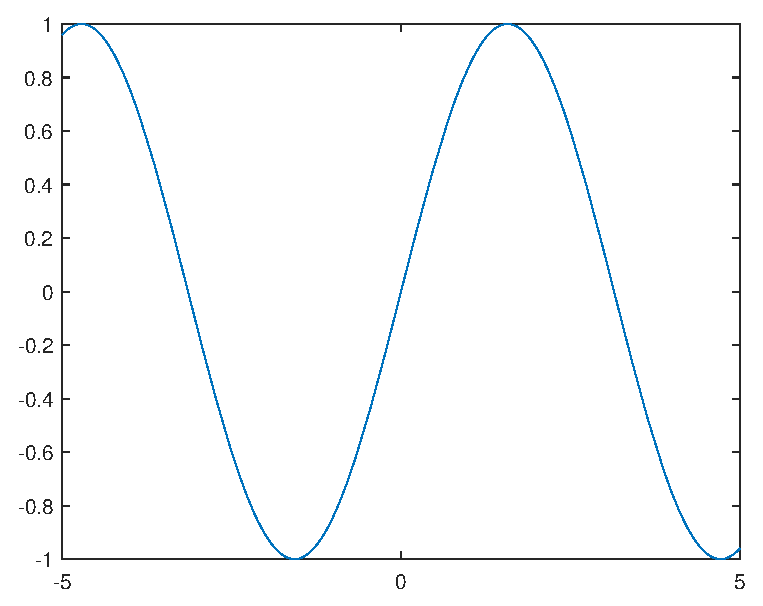
\includegraphics[width=7.2cm]{image1}
\caption{函数 $y=\sin(x)$ 的图像}\label{fig:sinx}
\end{figure}

两个图左右并排放置,共用一个标题,如图~\ref{fig:image}.
\begin{figure}[htp!]
\centering
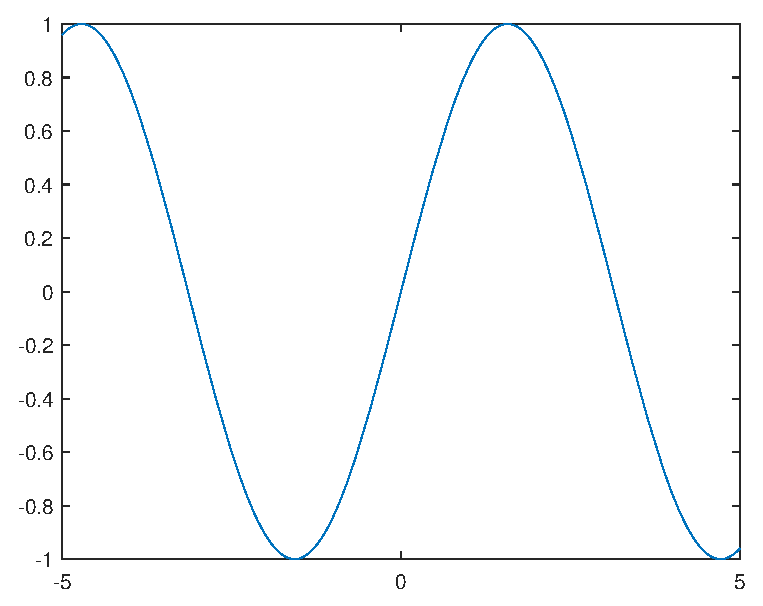
\includegraphics[width=0.45\linewidth]{image1}
\hfill
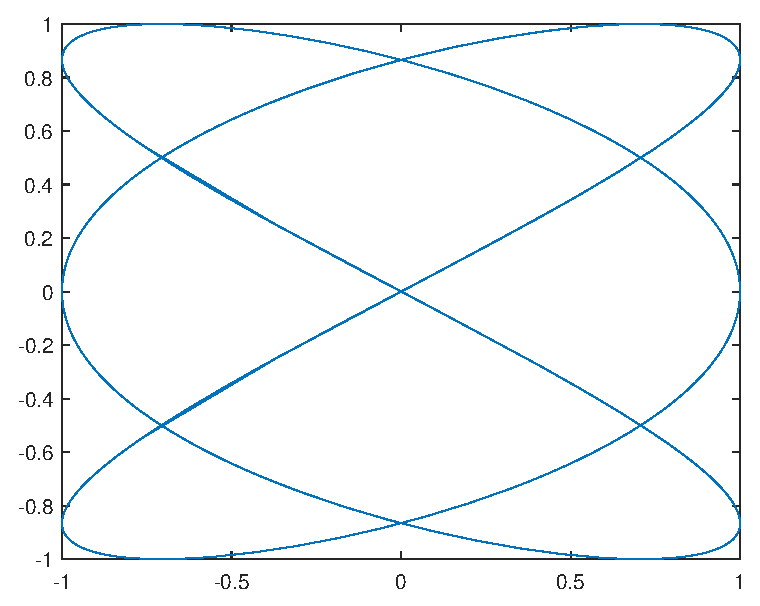
\includegraphics[width=0.45\linewidth]{image2}
\caption{左: 图一的描述;~ 右:图二的描述}
\label{fig:image}
\end{figure}

使用 minipage 排版并排插图,每个图都有单独的标题。通过 \verb|autoref| 引用图片: \autoref{fig:image1} 与 \autoref{fig:image2}.
\begin{figure}[htp!]
\begin{minipage}[t]{0.48\linewidth}
\centering
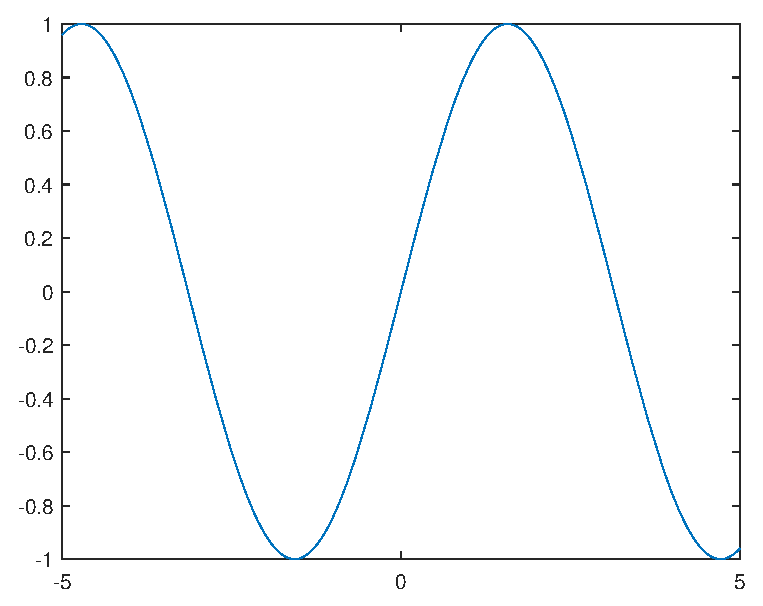
\includegraphics[width=0.9\linewidth]{image1}
\caption{图一的描述}
\label{fig:image1}
\end{minipage}
\hfill
\begin{minipage}[t]{0.48\linewidth}
\centering
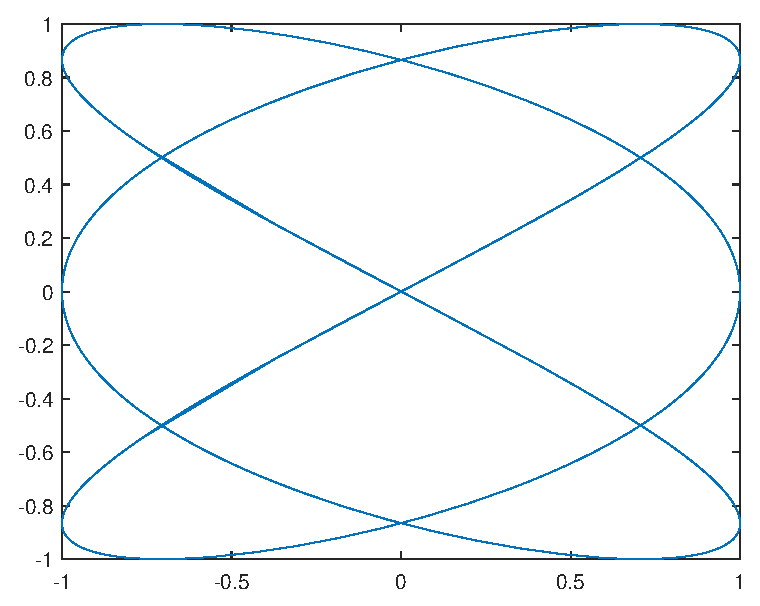
\includegraphics[width=0.9\linewidth]{image2}
\caption{图二的描述}
\label{fig:image2}
\end{minipage}
\end{figure}

使用 subfig 宏包实现多图并排,如图~\ref{fig:images}.
\begin{figure}[htp!]
\centering
\subfloat[Subcaption A]{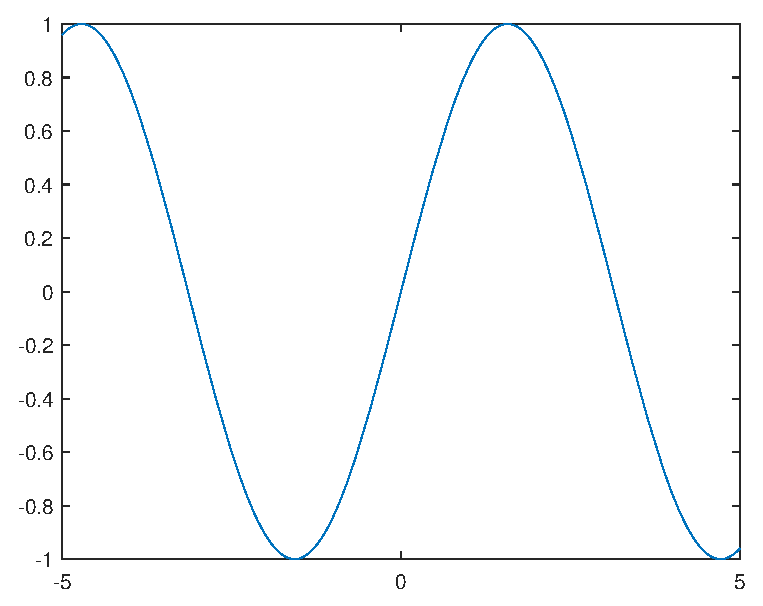
\includegraphics[width=0.45\linewidth]{image1}}
\hfill
\subfloat[Subcaption B]{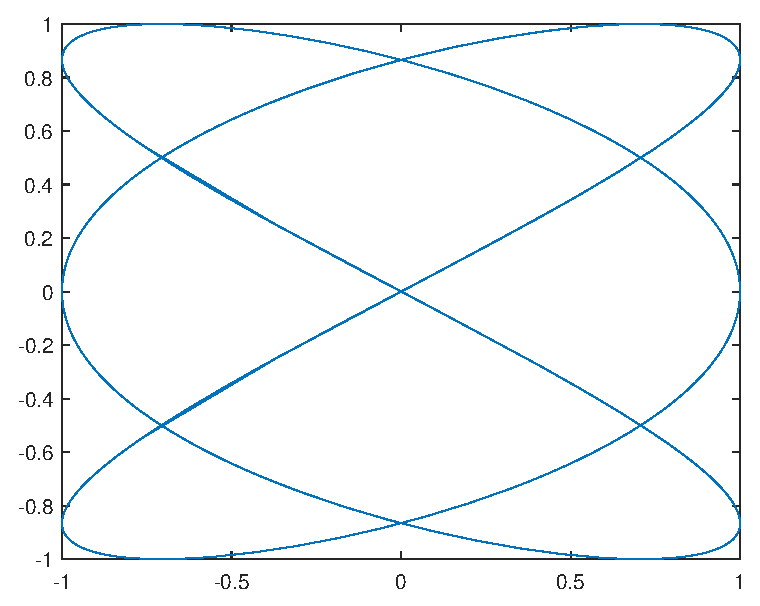
\includegraphics[width=0.45\linewidth]{image2}}
\caption{两个图并排子标题}
\label{fig:images}
\end{figure}

\subsubsection{表的使用}

LaTeX 的 table 环境是一个浮动体,与 figure 环境的排版方式类似。简单的表格可以使用三线表进行排版。

排版表格最基本的环境是 tabular 环境。如果想要控制表格行列间距,可使用命令 \verb|\tabcolsep| 和 \verb|\arraystretch|,它们分别控制列间距和行间距。例如,命令 \verb|\tabcolsep{10pt}| 表示列间距为 10pt,默认是 6pt,命令 \verb|\arraystretch{1.2}| 表示行间距为 1.2 倍,默认是 1 倍间距.

\textbf{表格示例}

使用 tabular 环境,如下表格: 表~\ref{tab:foo}。通过 \verb|autoref| 引用表格: \autoref{tab:foo}.

\begin{table}[htp!]
\centering
\setlength{\tabcolsep}{12pt}  % 6pt standard
\renewcommand{\arraystretch}{1.2}
\caption{学术活动安排样例}
\label{tab:foo}
\begin{tabular}{|c|c|c|c|}
\hline
\textbf{日期}  & \textbf{地点} & \textbf{活动名称} & \textbf{备注} \\ \hline
2024年8月1日      & 上海       & 学术研讨会      & 主题:人工智能 \\ \hline
2024年8月15日    & 北京       & 学术交流会      & 重点:数学建模 \\ \hline
2024年9月1日      & 深圳       & 研究研讨会      & 主题:数据科学 \\ \hline
2024年10月15日  & 广州       & 创新论坛         & 重点:科技创新 \\ \hline
\end{tabular}
\end{table}

\subsection{存在的问题}

内容

\renewcommand{\bibname}{\color{black}\normalfont\normalsize\bfseries 参考文献}

%============== 参考文献 ==============%

% 生成参考文献, 两种方式任选一种

% 第一种方式, 使用 bib 文件
%\nocite{*}  % 可以显示全部参考文献
\bibliography{reference}



% New section
\section{\textbf{项目的研究内容、研究目标,以及拟解决的关键科学问题}(此部分为重点阐述内容)\textbf{;}}

\section{\textbf{拟采取的研究方案及可行性分析}(包括研究方法、技术路线、实验手段、关键技术等说明);}

\section{\textbf{本项目的特色与创新之处;}}

\section{\textbf{年度研究计划及预期研究结果}\kern0.2em(包括拟组织的重要学术交流活动、国际合作与交流计划等)。}

\chapter{\textbf{研究基础与工作条件}}
\section{\textbf{研究基础}\kern0.2em(与本项目相关的研究工作积累和已取得的研究工作成绩);}

\section{\textbf{工作条件}\kern0.2em(包括已具备的实验条件,\kern0.2em 尚缺少的实验条件和拟解决的途径,包括利用国家实验室、全国重点实验室和部门重点实验室等研究基地的计划与落实情况);}

\section{\textbf{正在承担的与本项目相关的科研项目情况}\kern0.2em(申请人正在承担的与本项目相关的科研项目情况,包括国家自然科学基金的项目和国家其他科技计划项目,\kern0.1em 要注明项目的资助机构、\kern0.1em 项目类别、\kern0.1em 批准号、项目名称、获资助金额、起止年月、与本项目的关系及负责的内容等);\!\!\!}

\section{\textbf{完成国家自然科学基金项目情况}\kern0.2em(对申请人负责的前一个已资助期满的科学基金项目(项目名称及批准号)完成情况、后续研究进展及与本申请项目的关系加以详细说明。另附该项目的研究工作总结摘要(限 500 字)和相关成果详细目录)。}

\chapter{\textbf{其他需要说明的情况}}
\section{申请人同年申请不同类型的国家自然科学基金项目情况\kern0.2em(列明同年申请的其他项目的项目类型、项目名称信息,并说明与本项目之间的区别与联系;已收到自然科学基金委不予受理或不予资助决定的,无需列出)。}

\section{具有高级专业技术职务\kern0.2em(职称)\kern0.2em 的申请人是否存在同年申请或者参与申请国家自然科学基金项目的单位不一致的情况;如存在上述情况,列明所涉及人员的姓名,申请或参与申请的其他项目的项目类型、项目名称、单位名称、上述人员在该项目中是申请人还是参与者,并说明单位不一致原因。}

\section{具有高级专业技术职务\kern0.2em(职称)\kern0.2em 的申请人是否存在与正在承担的国家自然科学基金项目的单位不一致的情况;如存在上述情况,列明所涉及人员的姓名,正在承担项目的批准号、项目类型、项目名称、单位名称、起止年月,并说明单位不一致原因。}

\section{同年以不同专业技术职务\kern0.2em(职称)\kern0.2em 申请或参与申请科学基金项目的情况(应详细说明原因)。}

\section{其他。}



\end{document}

